\documentclass{standalone}
\usepackage{tikz}
\usetikzlibrary{patterns, positioning}
\usepackage[sfdefault]{ClearSans} %% option 'sfdefault' activates Clear Sans as the default text font
\usepackage[T1]{fontenc}

\begin{document}
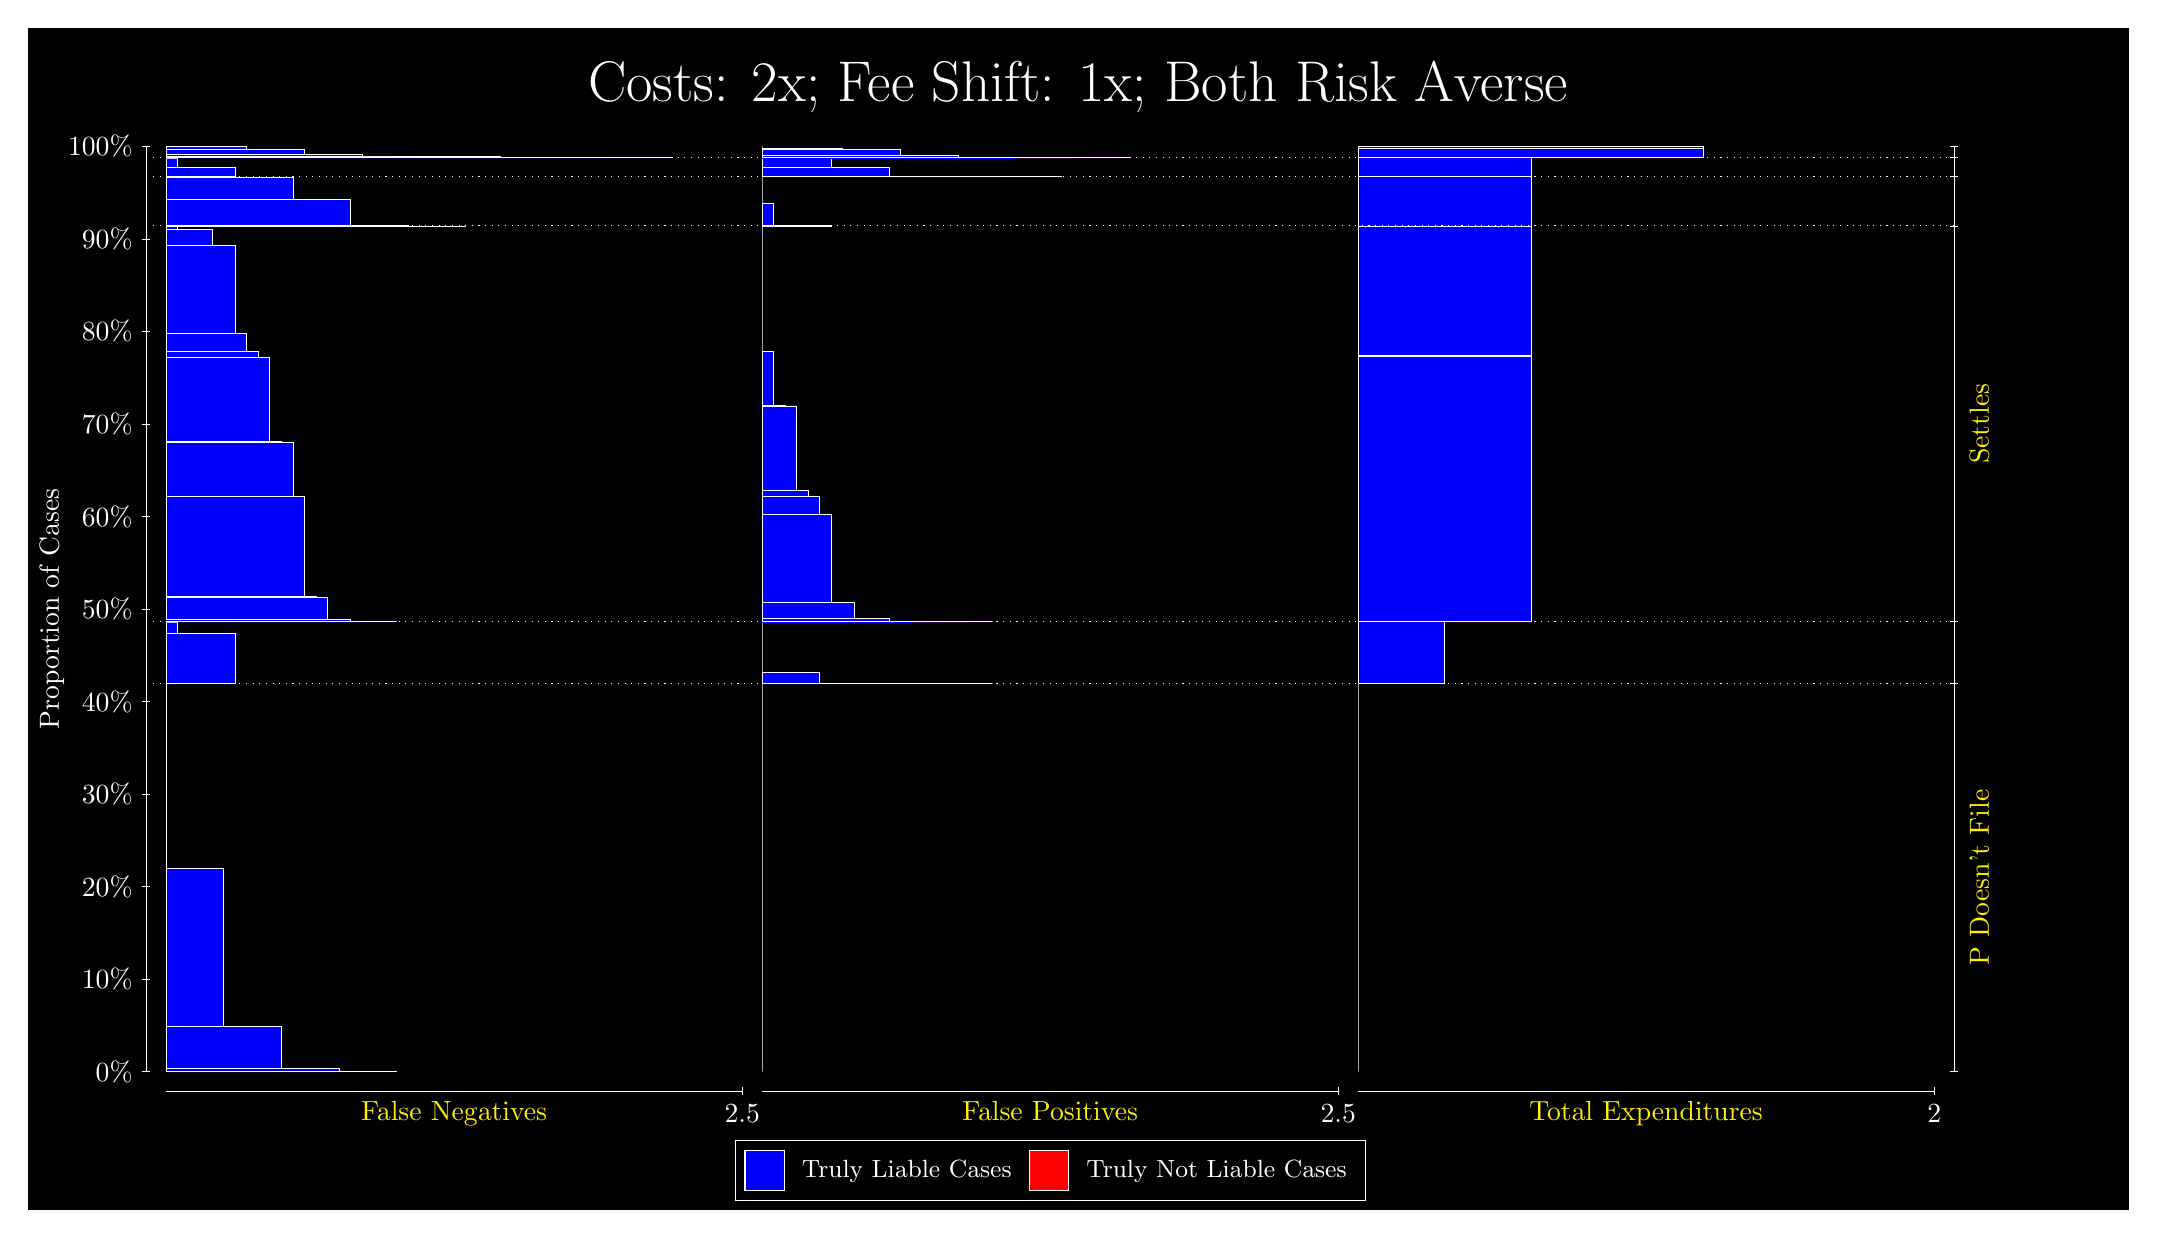
\begin{tikzpicture}
\draw[fill=black] (0,0) rectangle (26.667,15);
\draw[text=white] (0,13.5) rectangle (26.667,15) node[midway] {\huge Costs: 2x; Fee Shift: 1x; Both Risk Averse};
\draw[white, very thin] (1.5,1.75) -- (1.5,13.5);
\node[rotate=90, text=white, anchor=center] at (0.3, 7.625) {Proportion of Cases};
\draw[white, very thin] (1.45,1.75) -- (1.55,1.75);
\node[text=white, anchor=east] at (1.45, 1.75) {0\%};
\draw[white, very thin] (1.45,2.925) -- (1.55,2.925);
\node[text=white, anchor=east] at (1.45, 2.925) {10\%};
\draw[white, very thin] (1.45,4.1) -- (1.55,4.1);
\node[text=white, anchor=east] at (1.45, 4.1) {20\%};
\draw[white, very thin] (1.45,5.275) -- (1.55,5.275);
\node[text=white, anchor=east] at (1.45, 5.275) {30\%};
\draw[white, very thin] (1.45,6.45) -- (1.55,6.45);
\node[text=white, anchor=east] at (1.45, 6.45) {40\%};
\draw[white, very thin] (1.45,7.625) -- (1.55,7.625);
\node[text=white, anchor=east] at (1.45, 7.625) {50\%};
\draw[white, very thin] (1.45,8.8) -- (1.55,8.8);
\node[text=white, anchor=east] at (1.45, 8.8) {60\%};
\draw[white, very thin] (1.45,9.975) -- (1.55,9.975);
\node[text=white, anchor=east] at (1.45, 9.975) {70\%};
\draw[white, very thin] (1.45,11.15) -- (1.55,11.15);
\node[text=white, anchor=east] at (1.45, 11.15) {80\%};
\draw[white, very thin] (1.45,12.325) -- (1.55,12.325);
\node[text=white, anchor=east] at (1.45, 12.325) {90\%};
\draw[white, very thin] (1.45,13.5) -- (1.55,13.5);
\node[text=white, anchor=east] at (1.45, 13.5) {100\%};

\draw[white, very thin] (24.457,1.75) -- (24.457,13.5);
\draw[white, very thin] (24.407,1.75) -- (24.507,1.75);
\node[anchor=west] at (24.407, 1.75) {};
\draw[white, very thin] (24.407,6.6792) -- (24.507,6.6792);
\node[anchor=west] at (24.407, 6.6792) {};
\draw[white, very thin] (24.407,7.4621) -- (24.507,7.4621);
\node[anchor=west] at (24.407, 7.4621) {};
\draw[white, very thin] (24.407,12.49) -- (24.507,12.49);
\node[anchor=west] at (24.407, 12.49) {};
\draw[white, very thin] (24.407,13.115) -- (24.507,13.115);
\node[anchor=west] at (24.407, 13.115) {};
\draw[white, very thin] (24.407,13.356) -- (24.507,13.356);
\node[anchor=west] at (24.407, 13.356) {};
\draw[white, very thin] (24.407,13.5) -- (24.507,13.5);
\node[anchor=west] at (24.407, 13.5) {};

\draw[white, very thin, fill=blue] (1.75,1.75) rectangle (4.6775,1.7504);
\draw[white, very thin, fill=blue] (1.75,1.7504) rectangle (3.9457,1.7898);
\draw[white, very thin, fill=blue] (1.75,1.7898) rectangle (3.2138,2.3197);
\draw[white, very thin, fill=blue] (1.75,2.3197) rectangle (2.4819,4.3326);
\draw[white, very thin, fill=red] (1.75,4.3326) rectangle (1.75,4.3326);
\draw[white, very thin, fill=blue] (1.75,4.3326) rectangle (1.75,6.6792);
\draw[white, very thin, fill=blue] (1.75,6.6792) rectangle (2.6283,7.3204);
\draw[white, very thin, fill=blue] (1.75,7.3204) rectangle (1.8964,7.4582);
\draw[white, very thin, fill=red] (1.75,7.4582) rectangle (1.75,7.4582);
\draw[white, very thin, fill=blue] (1.75,7.4582) rectangle (1.75,7.4621);
\draw[white, very thin, fill=blue] (1.75,7.4621) rectangle (4.6775,7.4621);
\draw[white, very thin, fill=blue] (1.75,7.4621) rectangle (4.3848,7.4621);
\draw[white, very thin, fill=blue] (1.75,7.4621) rectangle (4.092,7.4888);
\draw[white, very thin, fill=blue] (1.75,7.4888) rectangle (3.9457,7.4892);
\draw[white, very thin, fill=blue] (1.75,7.4892) rectangle (3.7993,7.7782);
\draw[white, very thin, fill=blue] (1.75,7.7782) rectangle (3.6529,7.7863);
\draw[white, very thin, fill=blue] (1.75,7.7863) rectangle (3.5065,9.0613);
\draw[white, very thin, fill=blue] (1.75,9.0613) rectangle (3.3602,9.7377);
\draw[white, very thin, fill=blue] (1.75,9.7377) rectangle (3.2138,9.7507);
\draw[white, very thin, fill=blue] (1.75,9.7507) rectangle (3.0674,10.826);
\draw[white, very thin, fill=blue] (1.75,10.826) rectangle (2.921,10.897);
\draw[white, very thin, fill=blue] (1.75,10.897) rectangle (2.7746,11.122);
\draw[white, very thin, fill=blue] (1.75,11.122) rectangle (2.6283,12.24);
\draw[white, very thin, fill=blue] (1.75,12.24) rectangle (2.4819,12.245);
\draw[white, very thin, fill=blue] (1.75,12.245) rectangle (2.3355,12.441);
\draw[white, very thin, fill=blue] (1.75,12.441) rectangle (2.1891,12.445);
\draw[white, very thin, fill=blue] (1.75,12.445) rectangle (2.0428,12.446);
\draw[white, very thin, fill=blue] (1.75,12.446) rectangle (1.8964,12.49);
\draw[white, very thin, fill=red] (1.75,12.49) rectangle (1.75,12.49);
\draw[white, very thin, fill=blue] (1.75,12.49) rectangle (1.75,12.49);
\draw[white, very thin, fill=blue] (1.75,12.49) rectangle (5.5558,12.49);
\draw[white, very thin, fill=blue] (1.75,12.49) rectangle (4.8239,12.498);
\draw[white, very thin, fill=blue] (1.75,12.498) rectangle (4.092,12.83);
\draw[white, very thin, fill=blue] (1.75,12.83) rectangle (3.3602,13.112);
\draw[white, very thin, fill=blue] (1.75,13.112) rectangle (2.6283,13.115);
\draw[white, very thin, fill=red] (1.75,13.115) rectangle (1.75,13.115);
\draw[white, very thin, fill=blue] (1.75,13.115) rectangle (2.6283,13.232);
\draw[white, very thin, fill=blue] (1.75,13.232) rectangle (1.8964,13.352);
\draw[white, very thin, fill=red] (1.75,13.352) rectangle (1.75,13.352);
\draw[white, very thin, fill=blue] (1.75,13.352) rectangle (1.75,13.356);
\draw[white, very thin, fill=blue] (1.75,13.356) rectangle (8.1906,13.356);
\draw[white, very thin, fill=blue] (1.75,13.356) rectangle (7.4587,13.356);
\draw[white, very thin, fill=blue] (1.75,13.356) rectangle (6.7268,13.36);
\draw[white, very thin, fill=blue] (1.75,13.36) rectangle (5.9949,13.376);
\draw[white, very thin, fill=blue] (1.75,13.376) rectangle (5.7022,13.376);
\draw[white, very thin, fill=blue] (1.75,13.376) rectangle (5.2631,13.377);
\draw[white, very thin, fill=blue] (1.75,13.377) rectangle (4.9703,13.377);
\draw[white, very thin, fill=blue] (1.75,13.377) rectangle (4.5312,13.377);
\draw[white, very thin, fill=blue] (1.75,13.377) rectangle (4.2384,13.395);
\draw[white, very thin, fill=blue] (1.75,13.395) rectangle (3.7993,13.395);
\draw[white, very thin, fill=blue] (1.75,13.395) rectangle (3.5065,13.465);
\draw[white, very thin, fill=blue] (1.75,13.465) rectangle (2.7746,13.498);
\draw[white, very thin, fill=blue] (1.75,13.498) rectangle (2.0428,13.5);
\draw[white, very thin, fill=red] (1.75,13.5) rectangle (1.75,13.5);
\draw[white, very thin, fill=blue] (1.75,13.5) rectangle (1.75,13.5);
\draw[white, very thin, fill=red] (9.3189,1.75) rectangle (9.3189,1.75);
\draw[white, very thin, fill=blue] (9.3189,1.75) rectangle (9.3189,6.6792);
\draw[white, very thin, fill=red] (9.3189,6.6792) rectangle (12.246,6.6792);
\draw[white, very thin, fill=blue] (9.3189,6.6792) rectangle (12.246,6.6792);
\draw[white, very thin, fill=blue] (9.3189,6.6792) rectangle (11.515,6.6792);
\draw[white, very thin, fill=blue] (9.3189,6.6792) rectangle (10.783,6.6831);
\draw[white, very thin, fill=blue] (9.3189,6.6831) rectangle (10.051,6.8209);
\draw[white, very thin, fill=blue] (9.3189,6.8209) rectangle (9.3189,7.4621);
\draw[white, very thin, fill=red] (9.3189,7.4621) rectangle (12.246,7.4621);
\draw[white, very thin, fill=blue] (9.3189,7.4621) rectangle (12.246,7.4621);
\draw[white, very thin, fill=red] (9.3189,7.4621) rectangle (11.954,7.4621);
\draw[white, very thin, fill=blue] (9.3189,7.4621) rectangle (11.954,7.4621);
\draw[white, very thin, fill=red] (9.3189,7.4621) rectangle (11.661,7.4621);
\draw[white, very thin, fill=blue] (9.3189,7.4621) rectangle (11.661,7.4621);
\draw[white, very thin, fill=blue] (9.3189,7.4621) rectangle (11.515,7.4621);
\draw[white, very thin, fill=red] (9.3189,7.4621) rectangle (11.368,7.4621);
\draw[white, very thin, fill=blue] (9.3189,7.4621) rectangle (11.368,7.4621);
\draw[white, very thin, fill=blue] (9.3189,7.4621) rectangle (11.222,7.4624);
\draw[white, very thin, fill=red] (9.3189,7.4624) rectangle (11.075,7.4624);
\draw[white, very thin, fill=blue] (9.3189,7.4624) rectangle (11.075,7.4624);
\draw[white, very thin, fill=blue] (9.3189,7.4624) rectangle (10.929,7.5063);
\draw[white, very thin, fill=blue] (9.3189,7.5063) rectangle (10.783,7.5074);
\draw[white, very thin, fill=blue] (9.3189,7.5074) rectangle (10.636,7.5109);
\draw[white, very thin, fill=blue] (9.3189,7.5109) rectangle (10.49,7.7067);
\draw[white, very thin, fill=blue] (9.3189,7.7067) rectangle (10.344,7.7121);
\draw[white, very thin, fill=blue] (9.3189,7.7121) rectangle (10.197,8.8301);
\draw[white, very thin, fill=blue] (9.3189,8.8301) rectangle (10.051,9.0555);
\draw[white, very thin, fill=blue] (9.3189,9.0555) rectangle (9.9044,9.1258);
\draw[white, very thin, fill=blue] (9.3189,9.1258) rectangle (9.758,10.201);
\draw[white, very thin, fill=blue] (9.3189,10.201) rectangle (9.6116,10.214);
\draw[white, very thin, fill=blue] (9.3189,10.214) rectangle (9.4652,10.891);
\draw[white, very thin, fill=blue] (9.3189,10.891) rectangle (9.3189,12.49);
\draw[white, very thin, fill=red] (9.3189,12.49) rectangle (10.197,12.49);
\draw[white, very thin, fill=blue] (9.3189,12.49) rectangle (10.197,12.493);
\draw[white, very thin, fill=blue] (9.3189,12.493) rectangle (9.4652,12.775);
\draw[white, very thin, fill=blue] (9.3189,12.775) rectangle (9.3189,13.115);
\draw[white, very thin, fill=red] (9.3189,13.115) rectangle (13.125,13.115);
\draw[white, very thin, fill=blue] (9.3189,13.115) rectangle (13.125,13.115);
\draw[white, very thin, fill=blue] (9.3189,13.115) rectangle (12.393,13.115);
\draw[white, very thin, fill=blue] (9.3189,13.115) rectangle (11.661,13.12);
\draw[white, very thin, fill=blue] (9.3189,13.12) rectangle (10.929,13.24);
\draw[white, very thin, fill=blue] (9.3189,13.24) rectangle (10.197,13.356);
\draw[white, very thin, fill=red] (9.3189,13.356) rectangle (14.003,13.356);
\draw[white, very thin, fill=blue] (9.3189,13.356) rectangle (14.003,13.356);
\draw[white, very thin, fill=red] (9.3189,13.356) rectangle (13.271,13.356);
\draw[white, very thin, fill=blue] (9.3189,13.356) rectangle (13.271,13.356);
\draw[white, very thin, fill=red] (9.3189,13.356) rectangle (12.539,13.356);
\draw[white, very thin, fill=blue] (9.3189,13.356) rectangle (12.539,13.358);
\draw[white, very thin, fill=blue] (9.3189,13.358) rectangle (11.807,13.391);
\draw[white, very thin, fill=red] (9.3189,13.391) rectangle (11.807,13.391);
\draw[white, very thin, fill=blue] (9.3189,13.391) rectangle (11.807,13.391);
\draw[white, very thin, fill=blue] (9.3189,13.391) rectangle (11.075,13.461);
\draw[white, very thin, fill=blue] (9.3189,13.461) rectangle (11.075,13.462);
\draw[white, very thin, fill=red] (9.3189,13.462) rectangle (10.783,13.462);
\draw[white, very thin, fill=blue] (9.3189,13.462) rectangle (10.783,13.462);
\draw[white, very thin, fill=blue] (9.3189,13.462) rectangle (10.344,13.47);
\draw[white, very thin, fill=blue] (9.3189,13.47) rectangle (10.344,13.479);
\draw[white, very thin, fill=red] (9.3189,13.479) rectangle (10.051,13.479);
\draw[white, very thin, fill=blue] (9.3189,13.479) rectangle (10.051,13.479);
\draw[white, very thin, fill=blue] (9.3189,13.479) rectangle (9.6116,13.479);
\draw[white, very thin, fill=blue] (9.3189,13.479) rectangle (9.6116,13.479);
\draw[white, very thin, fill=red] (9.3189,13.479) rectangle (9.3189,13.479);
\draw[white, very thin, fill=blue] (9.3189,13.479) rectangle (9.3189,13.5);
\draw[white, very thin, fill=red] (16.888,1.75) rectangle (16.888,1.75);
\draw[white, very thin, fill=blue] (16.888,1.75) rectangle (16.888,6.6792);
\draw[white, very thin, fill=red] (16.888,6.6792) rectangle (17.986,6.6792);
\draw[white, very thin, fill=blue] (16.888,6.6792) rectangle (17.986,7.4621);
\draw[white, very thin, fill=red] (16.888,7.4621) rectangle (19.083,7.4621);
\draw[white, very thin, fill=blue] (16.888,7.4621) rectangle (19.083,10.829);
\draw[white, very thin, fill=red] (16.888,10.829) rectangle (19.083,10.829);
\draw[white, very thin, fill=blue] (16.888,10.829) rectangle (19.083,10.847);
\draw[white, very thin, fill=red] (16.888,10.847) rectangle (19.083,10.847);
\draw[white, very thin, fill=blue] (16.888,10.847) rectangle (19.083,12.49);
\draw[white, very thin, fill=red] (16.888,12.49) rectangle (19.083,12.49);
\draw[white, very thin, fill=blue] (16.888,12.49) rectangle (19.083,13.115);
\draw[white, very thin, fill=red] (16.888,13.115) rectangle (19.083,13.115);
\draw[white, very thin, fill=blue] (16.888,13.115) rectangle (19.083,13.356);
\draw[white, very thin, fill=red] (16.888,13.356) rectangle (21.279,13.356);
\draw[white, very thin, fill=blue] (16.888,13.356) rectangle (21.279,13.469);
\draw[white, very thin, fill=red] (16.888,13.469) rectangle (21.279,13.469);
\draw[white, very thin, fill=blue] (16.888,13.469) rectangle (21.279,13.5);
\draw[white, dotted] (1.5,6.6792) -- (24.457,6.6792);
\draw[white, dotted] (1.5,7.4621) -- (24.457,7.4621);
\draw[white, dotted] (1.5,12.49) -- (24.457,12.49);
\draw[white, dotted] (1.5,13.115) -- (24.457,13.115);
\draw[white, dotted] (1.5,13.356) -- (24.457,13.356);
\draw[white, very thin] (1.75,1.5) -- (9.0689,1.5);
\node[text=yellow, anchor=north] at (5.4094, 1.5) {False Negatives};
\draw[white, very thin] (9.0689,1.45) -- (9.0689,1.55);
\node[text=white, anchor=north] at (9.0689, 1.45) {2.5};

\draw[white, very thin] (9.3189,1.5) -- (16.638,1.5);
\node[text=yellow, anchor=north] at (12.978, 1.5) {False Positives};
\draw[white, very thin] (16.638,1.45) -- (16.638,1.55);
\node[text=white, anchor=north] at (16.638, 1.45) {2.5};

\draw[white, very thin] (16.888,1.5) -- (24.207,1.5);
\node[text=yellow, anchor=north] at (20.547, 1.5) {Total Expenditures};
\draw[white, very thin] (24.207,1.45) -- (24.207,1.55);
\node[text=white, anchor=north] at (24.207, 1.45) {2};

\node[text=yellow, centered, rotate=90] at (24.777, 4.2146) {P Doesn't File};

\node[text=yellow, centered, rotate=90] at (24.777, 9.976) {Settles};




\draw (12.978300999999998,1.5) node[draw=none] (baseCoordinate) {};
\begin{scope}[align=center]
        \matrix[scale=0.5, draw=white, below=0.5cm of baseCoordinate, nodes={draw}, column sep=0.1cm]{
            \node[rectangle, draw, minimum width=0.5cm, minimum height=0.5cm, fill=blue] {}; &
            \node[draw=none, font=\small, text=white] (B) {Truly Liable Cases}; &
            \node[rectangle, draw, minimum width=0.5cm, minimum height=0.5cm, fill=red] {}; &
            \node[draw=none, font=\small, text=white] (B) {Truly Not Liable Cases}; \\
            };
\end{scope}

\end{tikzpicture}
\end{document}